% This must be in the first 5 lines to tell arXiv to use pdfLaTeX, which is strongly recommended.
\pdfoutput=1
% In particular, the hyperref package requires pdfLaTeX in order to break URLs across lines.

\documentclass[11pt]{article}

% Remove the "guidelines" option to generate the final version.
%\usepackage[guidelines]{nlpreport} % show guidelines
\usepackage[]{nlpreport} % hide guidelines


% Standard package includes
\usepackage{times}
\usepackage{latexsym}
% For proper rendering and hyphenation of words containing Latin characters (including in bib files)
\usepackage[T1]{fontenc}
% For Vietnamese characters
% \usepackage[T5]{fontenc}
% See https://www.latex-project.org/help/documentation/encguide.pdf for other character sets

% This assumes your files are encoded as UTF8
\usepackage[utf8]{inputenc}

% This is not strictly necessary, and may be commented out,
% but it will improve the layout of the manuscript,
% and will typically save some space.
\usepackage{microtype}
\usepackage{graphicx}
\usepackage{hyperref}
\usepackage{amsmath}
\usepackage{mathtools}
\usepackage{multirow}
\usepackage{listings}
\usepackage{xcolor}
\usepackage{booktabs} % for tables
\usepackage{caption}





% THE pdfinfo Title AND Author ARE NOT NECESSARY, THEY ARE METADATA FOR THE FINAL PDF FILE
\hypersetup{pdfinfo={
Title={Assignment 2},
Author={Jane Smith \& John Doe}
}}
%\setcounter{secnumdepth}{0}  
 \begin{document}
%
\title{Assignment 2\\
\explanation{\rm Substitute the $\uparrow$ title $\uparrow$ with your project's title, or with Assignment 1 / 2\\ \smallskip}
% subtitle:
}
\author{Faharad Bayrami,
Gianluca Di Mauro,
Kaan Molla
\and
Leonardo Monti\\
Master's Degree in Artificial Intelligence, University of Bologna\\
\{ farhad.bayrami, gianluca.dimauro, mahmutkaan.molla, leonardo.monti3 \}@studio.unibo.it
}
\maketitle


\attention{DO NOT MODIFY THIS TEMPLATE - EXCEPT, OF COURSE FOR TITLE, SUBTITLE AND AUTHORS.\\ IN THE FINAL VERSION, IN THE \LaTeX\ SOURCE REMOVE THE \texttt{guidelines} OPTION FROM  \texttt{$\backslash$usepackage[guidelines]\{nlpreport\}}.
}

\begin{abstract}
%\begin{quote}

\explanation{
The abstract is very brief summary of your report. Try to keep it no longer than 15-20 lines at most. Write your objective, your approach, and your main observations (what are the findings that make this report worthwhile reading?)}
Multi-label text classification using pre-trained models, like BERT, has been a task of major interest in the last years.
This report delves into the exploration of classification of arguments on inherent human values underlying natural language arguments, with a specific emphasis on higher-order values such as "Openness to change," "Self-enhancement," "Conservation," and "Self-transcendence".
%\end{quote}
\end{abstract}

\attention{\textcolor{red}{NOTICE: THIS REPORT'S LENGTH MUST RESPECT THE FOLLOWING PAGE LIMITS: \begin{itemize}
    \item ASSIGNMENT: \textbf{2 PAGES} 
    \item NLP PROJECT OR PROJECT WORK: \textbf{8 PAGES}
    \item COMBINED NLP PROJECT + PW: \textbf{12 PAGES}
\end{itemize}  PLUS LINKS, REFERENCES AND APPENDICES.\\ 
THIS MEANS THAT YOU CANNOT FILL ALL SECTIONS TO MAXIMUM LENGTH. IT ALSO MEANS THAT, QUITE POSSIBLY, YOU WILL HAVE TO LEAVE OUT OF THE REPORT PART OF THE WORK YOU HAVE DONE OR OBSERVATIONS YOU HAVE. THIS IS NORMAL: THE REPORT SHOULD EMPHASIZE WHAT IS MOST SIGNIFICANT, NOTEWORTHY, AND REFER TO THE NOTEBOOK FOR ANYTHING ELSE.\\ 
FOR ANY OTHER ASPECT OF YOUR WORK THAT YOU WOULD LIKE TO EMPHASIZE BUT CANNOT EXPLAIN HERE FOR LACK OF SPACE, FEEL FREE TO ADD COMMENTS IN THE NOTEBOOK.\\ 
INTERESTING TEXT EXAMPLES THAT EXCEED THE MAXIMUM LENGTH OF THE REPORT CAN BE PLACED IN A DEDICATED APPENDIX AFTER THE REFERENCES.}}


\section{Introduction}
\label{sec:introduction}
\attention{MAX 1 COLUMN FOR ASSIGNMENT REPORTS / 2 COLUMNS FOR PROJECT OR PW / 3 FOR COMBINED REPORTS.}

\explanation{
The Introduction is an executive summary, which you can think of as an extended abstract.  Start by writing a brief description of the problem you are tackling and why it is important. (Skip it if this is an assignment report).} 

\explanation{Then give a short overview of known/standard/possible approaches to that problems, if any, and what are their advantages/limitations.} 

\explanation{After that, discuss your approach, and motivate why you follow that approach. If you are drawing inspiration from an existing model, study, paper, textbook example, challenge, \dots, be sure to add all the necessary references~\cite{DBLP:journals/corr/abs-2204-02311,DBLP:conf/acl/LorenzoMN22,DBLP:conf/clef/AnticiBIIGR21,DBLP:conf/ijcai/NakovCHAEBPSM21,DBLP:conf/naacl/RottgerVHP22,DBLP:journals/toit/LippiT16}.\footnote{\href{https://en.wikipedia.org/wiki/The_Muppet_Show}{Add only what is relevant.}}}

\explanation{Next, give a brief summary of your experimental setup: how many experiments did you run on which dataset. Last, make a list of the main results or take-home lessons from your work.}

\attention{HERE AND EVERYWHERE ELSE: ALWAYS KEEP IN MIND THAT, CRUCIALLY, WHATEVER TEXT/CODE/FIGURES/IDEAS/... YOU TAKE FROM ELSEWHERE MUST BE CLEARLY IDENTIFIED AND PROPERLY REFERENCED IN THE REPORT.}
The main interest was in developing three different models able to correctly classify arguments on human values, basing the evaluation only on the arguments' conclusions for the first, then adding also the premises in the second one and finally including the stances in the third one, which express if the specific argument is "in favor of" or "against" the specific discussed topic. The approach was first to utilize an auto-model to better understand the problem, then we moved on a custom model, in order to better address all the requirements. Operating on a train dataset of only 5393 entries, some inaccuracies have been faced, anyway promising results were obtained especially by the second and the third model, with F1-scores up to "0.75".
\section{System description}
\label{sec:system}
\attention{MAX 1 COLUMN FOR ASSIGNMENT REPORTS / 4 COLUMNS FOR PROJECT OR PW / 6 FOR COMBINED REPORTS.}

\explanation{
Describe the system or systems you have implemented (architectures, pipelines, etc), and used to run your experiments. If you reuse parts of code written by others, be sure to make very clear your original contribution in terms of
\begin{itemize}
    \item architecture: is the architecture your design or did you take it from somewhere else
    \item coding: which parts of code are original or heavily adapted? adapted from existing sources? taken from external sources with minimal adaptations?
\end{itemize}
It is a good idea to add figures to illustrate your pipeline and/or architecture(s)
(see Figure~\ref{fig:architecture})
%
\begin{figure*}
    \centering
    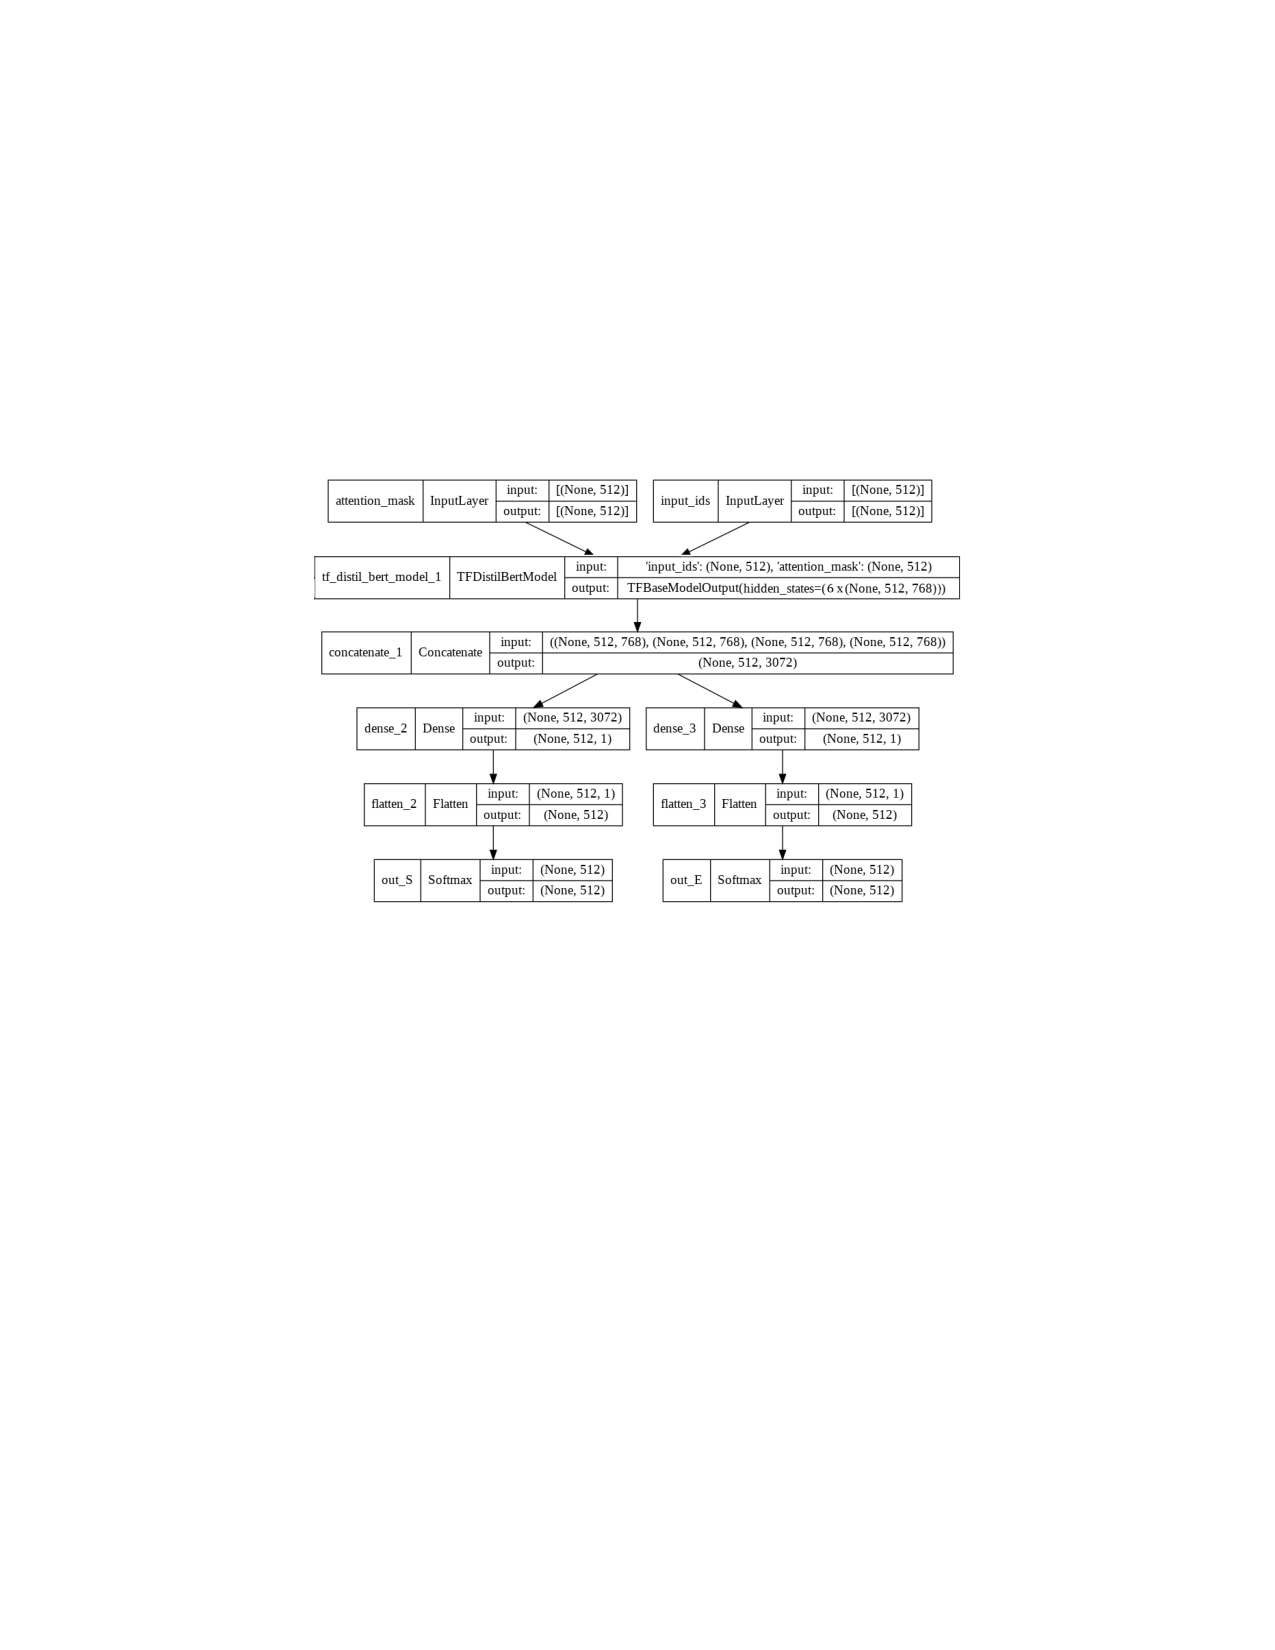
\includegraphics[width=\textwidth]{img/architecture.pdf}
    \caption{Model architecture}
    \label{fig:architecture}
\end{figure*}
}
The system runs entirely on Python. Six different datasets, three for arguments and three for labels, are downloaded and assembled into train, validation and test datasets. Then merging over categories is applied to obtain human values labels.
Two baseline models were used: a majority classifier and a random uniform classifier.
The aforementioned Bert based models, were all implemented on a pre-trained BertModel and for each, dataset tokenization, through bert-base uncased pre trained tokenizer, is applied with small differences.
Worthy of mention some trials using an Huggingface "Automodel-for-sequence-classification" ~\cite{wolf2020huggingfaces}. Despite decent results were obtained, switching to a custom model class was preferred.
Like tokenization functions, training and evaluation functions have been tailor-made to the models, allowing to better operate on different parameters, like the loss function, which will be discussed in the next section.
The models are implemented and trained using the Pytorch framework for reproducibility and
experimental reasons. 
The architecture mimics the one of Huggingface automodels, it includes the Bert model and a linear classifier. An additional value is stacked to the Bert output when the Stance is used for the classification.

\section{Experimental setup and results}
\label{sec:results}
\attention{MAX 1 COLUMN FOR ASSIGNMENT REPORTS / 3 COLUMNS FOR PROJECT OR PW / 5 FOR COMBINED REPORTS.}

\explanation{
Describe how you set up your experiments: which architectures/configurations you used, which hyper-parameters and what methods used to set them, which optimizers, metrics, etc.
\\
Then, \textbf{use tables} to summarize your your findings (numerical results) in validation and test. If you don't have experience with tables in \LaTeX, you might want to use \href{https://www.tablesgenerator.com/}{\LaTeX table generator} to quickly create a table template.
}
To train the model we opted for the AdamW optimizer, which allows to tune the Weight Decay parameter.
%, which didn't have great impact on the model.
Then BCEWithLogitsLoss was used as loss function, after some trials using instead F1, with poor results. This loss combines a Sigmoid layer and the BCELoss (Binary Cross Entropy) in one single class. This version is more numerically stable than using a plain Sigmoid followed by a BCELoss as, by combining the operations into one layer, we take advantage of the log-sum-exp trick for numerical stability~\cite{NEURIPS2019_9015}.
Due to train set class imbalance, applying weights to the loss function was beneficial. Weights were calculated using a custom function based on the square root of the inverse of the class frequency. In particular the first class is the least represented and a major weight of "1.666" was applied; other weights applied as follows: "1.529, 1.158, 1.188".
This ensured improvements in predicting the first class.
The last parameter needed for Adam to train the model is the learning rate. Initial tests with a learning rate of 2e-5 were done, following proven results~\cite{DBLP:conf/cncl/SunQXH19}. The best results on the less frequent classes were obtained that way. Further experiments were done raising the learning rate. Table~\ref{tab:table 2} shows the results for learning rates of 2e-5 and 3e-5.
Worth of attention the already mentioned Weight Decay, which didn't improve results, despite trying a wide range of values. All the results provided are averages over the results of three executions using different random seeds, to edge against training variability.
%The used seeds are "333", "666", "999".

\begin{table}[ht]
\centering
\begin{tabular}{|c| c c|}
\hline 
Classifier & Macro F1 & Per-Category F1 \\
\hline
 Uniform &  0.48 & [0.39, 0.41, 0.58, 0.58]\\
 Majority & 0.49  & [0.37, 0.46, 0.59, 0.56]\\
 \hline
\end{tabular}
\caption{Baselines' F1 Scores}
\label{tab:table 1}
\end{table}


%%%
%\begin{table}[ht]
%\centering
%\begin{tabular}{|c| c c c |}
%\hline 
%Learning Rate & C & C-P & C-P-S \\
%\hline
% 2e-5 & 0.67  & 0.73 & 0.73  \\
% 3e-5 & 0.64 & 0.75 & 0.74 \\
% \hline
%\end{tabular}
%\caption{Models' average Macro F1 Scores}
%\end{table}
%%%

\begin{table}[ht]
\centering
\begin{tabular}{|c| c c c c | c |}
\hline 
Model & OtC & SE & C & ST & Macro \\
\hline
 lr 2e-5 & & & & &\\
 C     & 0.40	& 0.59  & 0.85	& 0.85 & 0.67 \\
 C-P   & 0.57	& 0.67	& 0.85	& 0.85 & 0.73 \\
 C-P-S & 0.56	& 0.65	& 0.85	& 0.85 & 0.73 \\
 \hline
lr 3e-5 & & & & & \\
 C     & 0.26	& 0.62	&0.85	& 0.85 & 0.64 \\
 C-P   & 0.60	& 0.68	& 0.85	& 0.85 & 0.75 \\
 C-P-S & 0.56	& 0.68	& 0.85	& 0.85 & 0.74 \\
 


 \hline
\end{tabular}
\caption{Models' average F1 Scores per category and Macro}
\label{tab:table 2}
\end{table}





\section{Discussion}
\label{sec:discussion}
\attention{MAX 1.5 COLUMNS FOR ASSIGNMENT REPORTS / 3 COLUMNS FOR PROJECT / 4 FOR COMBINED REPORTS. ADDITIONAL EXAMPLES COULD BE PLACED IN AN APPENDIX AFTER THE REFERENCES IF THEY DO NOT FIT HERE.}



\explanation{
Here you should make your analysis of the results you obtained in your experiments. Your discussion should be structured in two parts: 
\begin{itemize}
    \item discussion of quantitative results (based on the metrics you have identified earlier; compare with baselines);
    \item error analysis: show some examples of odd/wrong/unwanted  outputs; reason about why you are getting those results, elaborate on what could/should be changed in future developments of this work.
\end{itemize}
}
Many experiments were made, allowing to progressively build a more well-suited model. First of all the two baseline models were tested; for both the random uniform classifier and the majority classifier, overall F1 score and per category F1 score were calculated, as shown in Table~\ref{tab:table 1}. Then, several tests were done using an auto-model, which produced unsatisfactory results, which are not reported not being relevant. On the other hand, the custom models surely performed better than both of them. The conclusion only model was the weakest of the three obtaining low F1 score values that are still better than the baselines. For the other two models the results improved which shows how including the premise was beneficial, while the stance didn't provide too much of a help to the models' accuracy. Results are reported in Table~\ref{tab:table 2}. In Figure~\ref{fig:graph} we compare the performances of the classifiers with the frequencies of the class in the training set. It is evident how the Bert model using only the conclusion with learning rate = 3e-5 overfits on the first category, that is the least represented. A similar issue is discussed in \cite{kiesel-etal-2022-identifying}. 

\begin{figure}
    %\centering
    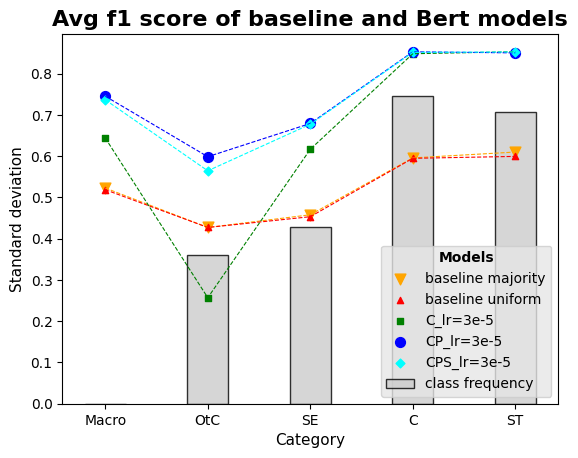
\includegraphics[scale=0.55]{img/output.png}
    \caption{Average F1 scores of Baselines and Bert Classifiers, compared with class frequencies for each category.}
    \label{fig:graph}
\end{figure}


\section{Conclusion}
\label{sec:conclusion}
\attention{MAX 1 COLUMN.}

\explanation{
In one or two paragraphs, recap your work and main results.
What did you observe? 
Did all go according to expectations? 
Was there anything surprising or worthwhile mentioning?
After that, discuss the main limitations of the solution you have implemented, and indicate promising directions for future improvement.
}
The implemented models performed quite well, considering the limited data and resources available. The first model was the weakest of the three, being more prone to overfitting especially on the first category.
The second model improved results by far, demonstrating that adding to the input arguments' conclusion was beneficial. Lastly for the third model, adding stance didn't provide a significant difference.
What emerged, as is shown in Figure 1, is some correlation between value frequencies and classifier performances, this may be due to dataset  being too small for training reliable classifiers on the infrequent values as suggested by \cite{kiesel-etal-2022-identifying}
The main limitations were surely encountered due to a very small training set in terms of entries, but also in length of arguments provided.
Possible future developments could consider further pre-training the bert model on the dataset, to suite the model to the specific implemented task as described by \cite{DBLP:conf/cncl/SunQXH19}



\section{Links to external resources}
All the materials of this assignments are available at the following 
\label{sec:links}
\attention{THIS SECTION IS OPTIONAL}
\explanation{
Insert here:
\begin{itemize}
    \item a link to your GitHub or any other public repo where one can find your code (only if you did not submit your code on Virtuale); 
    \item a link to your dataset (only for non-standard projects or project works).
\end{itemize}
}
 \href{https://github.com/luke1399/Assignment2}{GitHub repository} 

\attention{DO NOT INSERT CODE IN THIS REPORT}







\bibliography{nlpreport.bib}
\end{document}